\documentclass[languages_and_machines.tex]{subfiles}
\begin{document}

% \begin{frame}
%   \frametitle{Regular languages}

%   Language: Languages using arbitary repetition and optional elements.

%   Grammar: A \pro Yz or A \pro z (left-version).

%   Machine: Deterministic finite-state automaton.

% \end{frame}

\begin{frame}
  \frametitle{Deterministic finite-state automata}

  Example language: Multiples of 3 in binary notation

  \vspace{5mm}
  \pause

  Note that remainder can be computed if you slap on another digit.

  \begin{tabular}{l||p{4cm}|p{4cm}}
    remainder & after appending 0 & after appending 1 \\
    \(x \pmod 3\) & \(x.0 \pmod 3\) & \(x.1 \pmod 3\)
    \only<2>{
    \\ \hline \hline & &
    \\ \hline  & &
    \\ \hline  & &
    }
    \only<3>{
    \\ \hline \hline 0 & 0 & 1
    \\ \hline 1 & 2 & 0
    \\ \hline 2 & 1 & 2
    \\}
  \end{tabular}

\end{frame}

\begin{frame}
  \frametitle{Deterministic finite-state automata}

  \begin{tikzpicture}[->,>=stealth',shorten >=1pt,auto,node distance=2.8cm,semithick,ampersand replacement=\&]

  \node[accepting,initial,state] (s0)               {r = 0 \only<2>{\!\!*\!\!\!}\only<7>{\!\!*\!\!\!}\only<8>{\!\!*\!\!\!}\only<10>{\!\!*\!\!\!}};
  \node[state]                   (s1) [right of=s0] {r = 1 \only<4>{\!\!*\!\!\!}\only<5>{\!\!*\!\!\!}};
  \node[state]                   (s2) [right of=s1] {r = 2};

  \path (s0) edge [loop above   ] node {0 \only<9>{\!\!*\!\!\!}} (s0)
             edge [bend left= 45] node {1 \only<3>{\!\!*\!\!\!}} (s1)
        (s1) edge [bend left=-45] node {0} (s2)
             edge [bend left= 45] node {1 \only<6>{\!\!*\!\!\!}} (s0)
        (s2) edge [bend left=-45] node {0} (s1)
             edge [loop above   ] node {1} (s2)
  ;
  \end{tikzpicture}

  \only<2-4>{\textcolor{red}{1}10}
  \only<5-7>{1\textcolor{red}{1}0}
  \only<8-10>{11\textcolor{red}{0}}

\end{frame}

\begin{frame}
  \frametitle{Deterministic Finite-state Automata}

  \begin{block}{Definition}
    \textbf{Deterministic finite state automata} := \begin{itemize}
    \item \(S\): a finite set of states
    \item \(A \subseteq S\): a set of accepting states
    \item \(S_0 \in S\): an intial state
    \item \(\Sigma\): a finite alphabet
    \item \(f : S \times \Sigma \to S\): state-transition function
    \end{itemize}
  \end{block}
\end{frame}

\begin{frame}
  \frametitle{Nondeterministic Finite-state Automata}

  \begin{block}{Definition}
    \textbf{Nondeterministic finite state automata} := \begin{itemize}
    \item \(S\): a finite set of states
    \item \(A \subseteq S\): a set of accepting states
    \item \(S_0 \in S\): an intial state
    \item \(\Sigma\): a finite alphabet
    \item \(f : S \times (\Sigma \cup \textcolor{red}{\{\varepsilon\}}) \to \textcolor{red}{\powerset}(S)\): state-transition function
    \end{itemize}
  \end{block}

\end{frame}

\begin{frame}
  \frametitle{NFA}

  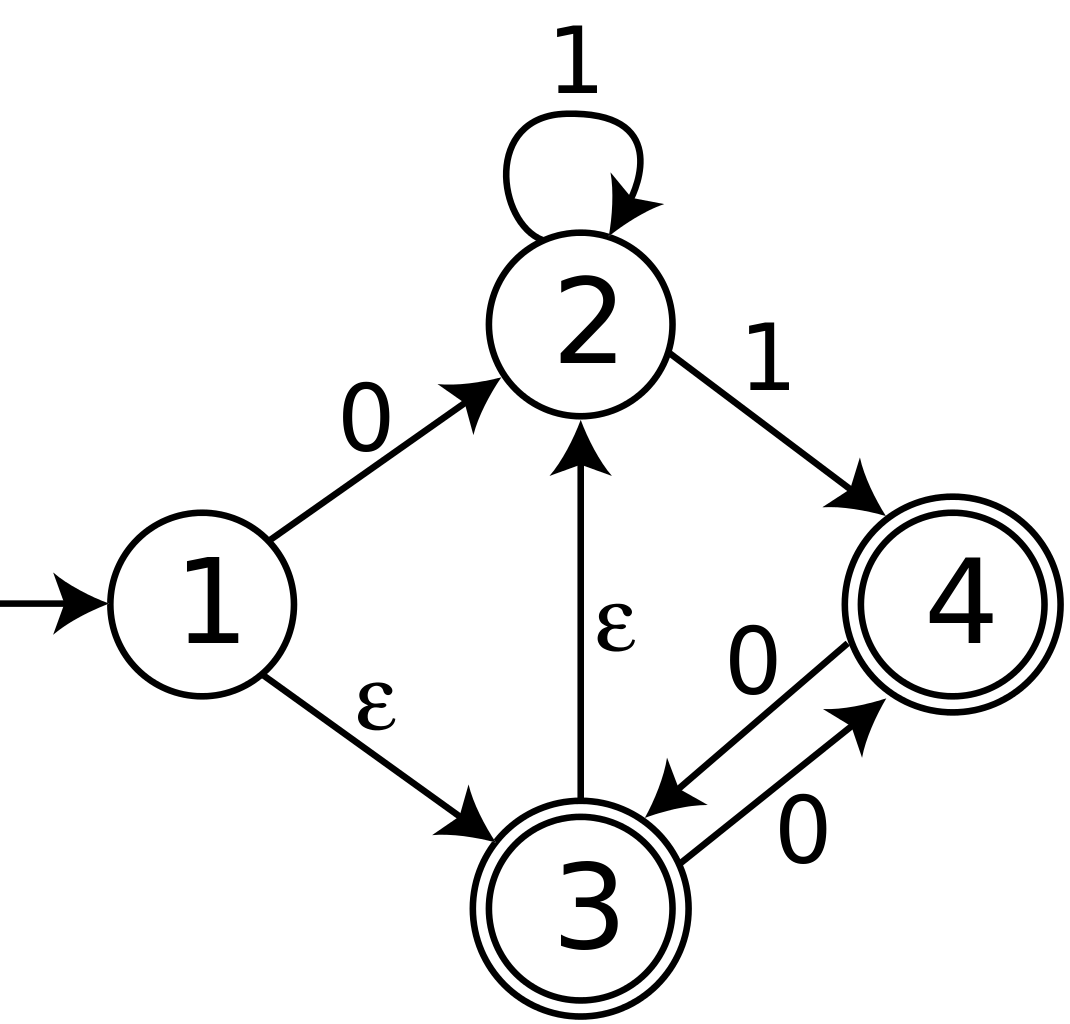
\includegraphics[width=0.4\textwidth]{nfa-powerset.png}

  {\tiny
    Figure from \href{https://commons.wikimedia.org/wiki/File:NFA-powerset-construction-example.svg}{WikiMedia}
  }
\end{frame}

\begin{frame}
  \frametitle{NFA \(\iff\) DFA}

  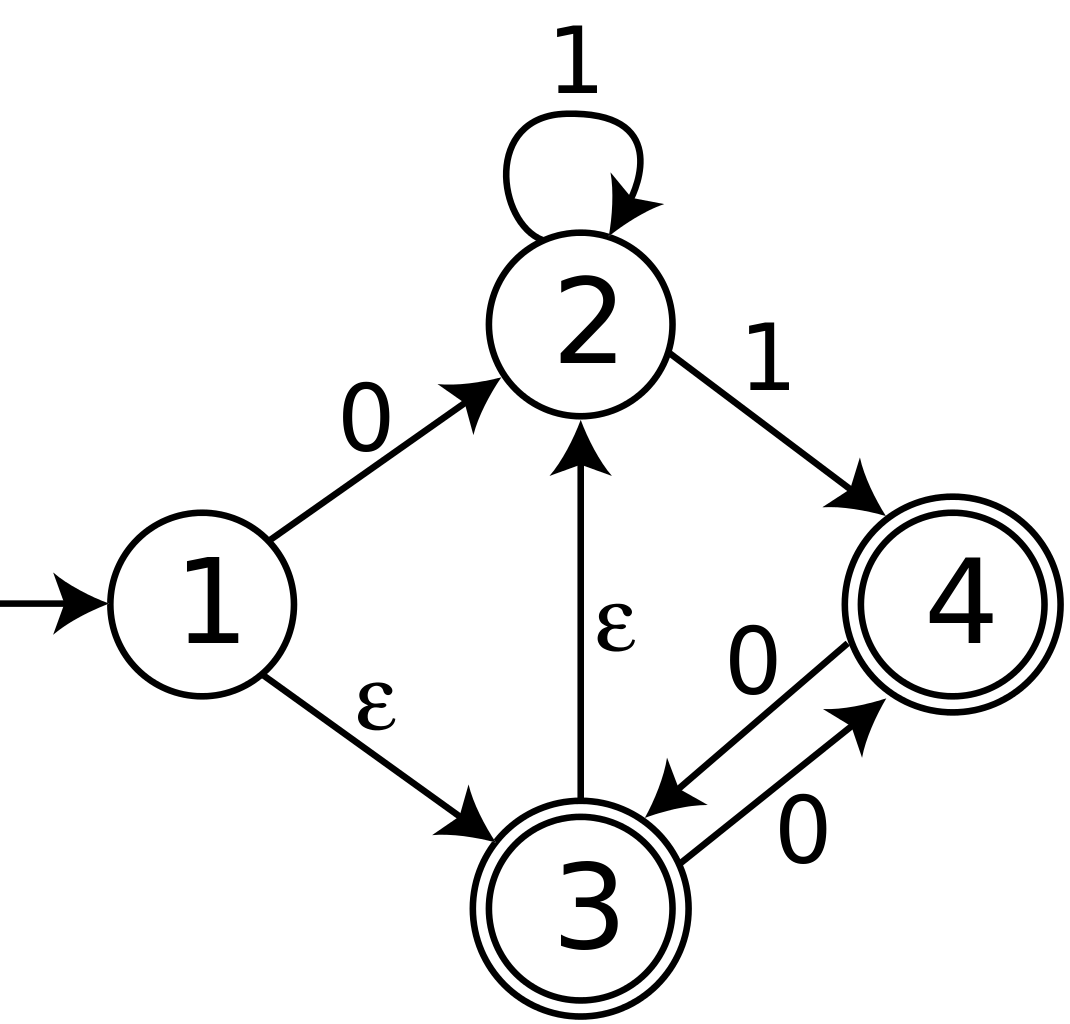
\includegraphics[width=0.48\textwidth]{nfa-powerset.png}
  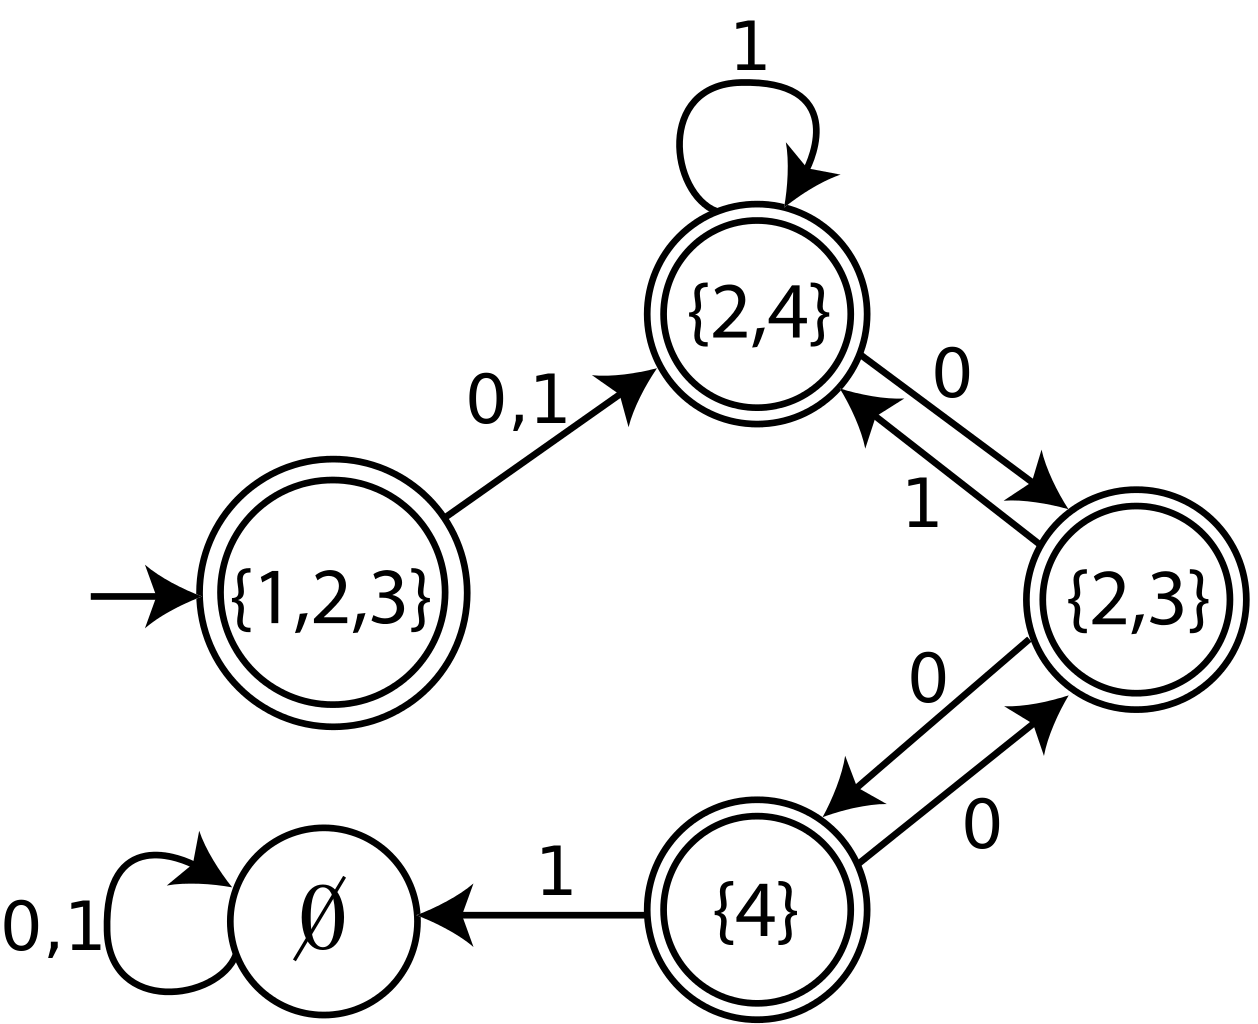
\includegraphics[width=0.48\textwidth]{dfa-powerset.png}

  \pause

  possibly \(n\) states \pro \(2^n\) states, worst-case.

  {\tiny
    Figure 1 from \href{https://commons.wikimedia.org/wiki/File:NFA-powerset-construction-example.svg}{WikiMedia}

    Figure 2 from \href{https://commons.wikimedia.org/wiki/File:DFA-powerset-construction-example.svg}{WikiMedia}
  }
\end{frame}

\begin{frame}
  \frametitle{Regular grammar}

  \begin{block}{Definition}
    \textbf{Regular grammar} := Languages where every rule is of the form A \pro \emptystr, A \pro aB (right-regular).
  \end{block}

  \pause

  Note: more than one rule could apply. A string is generated if any of these are valid.

  We can construct \(A \to a\) by \pause \(A \to a B\) and \(B \to \varepsilon\)

  Likewise \(A \to a_1 a_2 \dotsb a_n B\) by \pause \(A \to a_1 A_1\), \(A_1 \to a_2 A_2\), \(\dotsb\), \(A_n \to a_n B\).

\end{frame}

\begin{frame}
  \frametitle{Regular Grammar example}

  Example language: Multiples of 3 in binary notation

{\footnotesize
  \begin{tabular}{l||p{4cm}|p{4cm}}
    remainder & after appending 0 & after appending 1 \\
    \(x \pmod 3\) & \(x.0 \pmod 3\) & \(x.1 \pmod 3\)
    \\ \hline \hline 0 & 0 & 1
    \\ \hline 1 & 2 & 0
    \\ \hline 2 & 1 & 2
    \\
  \end{tabular}
  }

A \pro 0A \\
A \pro 1B \\
B \pro 0C \\
B \pro 1A \\
C \pro 0B \\
C \pro 1C \\
\pause
A \pro \emptystr \\
S \pro A \\

TODO: redraw DFA

A \pro 1B \pro 11A \pro 110A \pro 110
\end{frame}

\begin{frame}
  \frametitle{NFA \(\iff\) Regular Grammar}

  Transition,
  \begin{tikzpicture}[->,>=stealth',shorten >=1pt,auto,node distance=2.8cm,semithick,scale=0.2,every node={scale=0.2}]
  \node[state] (s0)               {A};
  \node[state] (s1) [right of=s0] {B};
  \path (s0) edge [bend right=-45] node {c} (s1);
  \end{tikzpicture},
  corresponds to rule,
  A \pro cB.

  Start state = starting symbol, ending states \pro \emptystr

  Useful for proofs.

\end{frame}

\begin{frame}
  \frametitle{Properties of Regular Languages}

  Languages with arbitrary repetition and optional elements.

  \pause

  Closed under complementation. \pause Proof: switch accepting and non-accepting states in DFA.

  \pause

  Closed under dis/conjunction. \pause Proof: consider cartesian product of two machines.

  \pause

  Closed under Kleene-*. \pause Proof: accepting state to start state with \emptystr transition

  \pause

  Algorithm to minimize (1979)

  \textbf{always halts; linear time}

\end{frame}

\begin{frame}
  \frametitle{Pumping lemma (1969)}

  Lemma: For all DFA with \(n\) states, for all strings, \(x \in L\) longer than \(n\), \(\ldots\)

  \pause

  Proof: \(\lvert x \rvert > n\), so visits a state twice (pigeon-hole).

  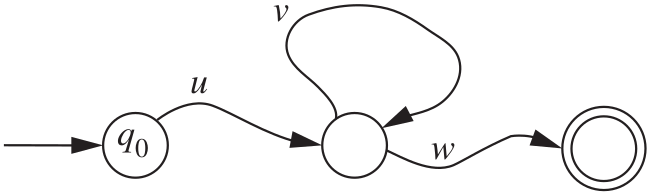
\includegraphics[width=0.4\textwidth]{pumping_lemma.png}

  \pause

  Now \(x\) can be decomposed into \(uvw\) where \(v\) can be repeated, so \(uv^iw \in L\) also.

Note that \(v\) is non-empty and \(\abs{uv} \leq n\).

    {\tiny Figure from ``Introduction to Languages and the Theory of Computation'' by John C. Martin}

\end{frame}

\begin{frame}
  \frametitle{Pumping lemma (1969)}

  Given a regular language, \(L\),

  There exists \(n \in \mathbb N\) such that \begin{itemize}
    \item For all \(x \in L\) and \(\abs{x} > n\)
      \begin{itemize}
      \item  There exists \(u, v, w\) where
        \begin{enumerate}
        \item \(x = uvw\)
        \item \(v \neq \varepsilon\)
        \item \(\abs{uv} \leq n\)
        \item \(uv^iw \in L\) for all \(i \in N\)
        \end{enumerate}
      \end{itemize}
    \end{itemize}
\end{frame}

\begin{frame}
  \frametitle{Pumping lemma example}

  \begin{tikzpicture}[->,>=stealth',shorten >=1pt,auto,node distance=2.8cm,semithick,ampersand replacement=\&,scale=0.5,every node/.style={scale=0.5}]

  \node[accepting,initial,state] (s0)               {r = 0};
  \node[state]                   (s1) [right of=s0] {r = 1};
  \node[state]                   (s2) [right of=s1] {r = 2};

  \path (s0) edge [loop above   ] node {0} (s0)
             edge [bend left= 45] node {1} (s1)
        (s1) edge [bend left=-45] node {0} (s2)
             edge [bend left= 45] node {1} (s0)
        (s2) edge [bend left=-45] node {0} (s1)
             edge [loop above   ] node {1} (s2)
  ;
  \end{tikzpicture}

  \begin{itemize}
  \item Let's try divisble-by-3 DFA for \(9 = 1001\).
  \pause
  \item We can pump the double-zeros. \(1(00)^n1\) is divisible by three.
  \pause
  \item Indeed \(1 + 2^{1 + 2n} \pmod 3 = 1 + (-1) = 0\).
  \end{itemize}
\end{frame}

\begin{frame}
  \frametitle{More difficult languages}

  \begin{itemize}
  \item \(L = \{a^n b^n : n \in \mathbb N\}\). \pause No substring can be pumped up.

    \pause

  \item Language of matched brackets (e.g. ``(())()'').
    \\\pause For every \(n\), no less than\(n\)-long substring of \((^n)^n\) can be pumped up.

    \pause

  \item Palindromes
    \\\pause For every \(n\), no less than \(n\)-long substring of \(a^n b^n\) can be pumped up.

    \pause

  \item Language where length of strings is not ``eventually linear''

  \item Challenge: \(L\) is not regular, but \(L^2\) is.

  \end{itemize}
\end{frame}

\end{document}
%%% Local Variables:
%%% mode: latex
%%% TeX-master: t
%%% End:
